\documentclass{article}

% Language setting
% Replace `english' with e.g. `spanish' to change the document language
%\usepackage[english,portuguese]{babel}
\usepackage[brazil]{babel}
\usepackage[utf8]{inputenc}

% Set page size and margins
% Replace `letterpaper' with `a4paper' for UK/EU standard size
\usepackage[a4paper,top=2cm,bottom=2cm,left=3cm,right=3cm,marginparwidth=1.75cm]{geometry}

% Useful packages
\usepackage{amsmath,amsthm,amsfonts,float}
\usepackage{graphicx}
\usepackage[colorlinks=true, allcolors=blue]{hyperref}

%\newenvironment{namebox}
%{\begin{flushleft}Nome: \underline{\hspace{6cm}}\end{flushleft}} % Adjust the length of the underline as needed

\newcommand{\na}{\mathbb{N}} % Set of integers
\newcommand{\naz}{\mathbb{N}_0} % Set of integers
\newcommand{\Z}{\mathbb{Z}} % Set of integers
\newcommand{\re}{\mathbb{R}} % Set of real numbers
\newcommand{\sinal}{\mathrm{sinal}} % Signal operador

\newcommand{\vp}{{\mathbf p}}
\newcommand{\vP}{{\mathbf P}}

\newcommand{\vpi}{{\boldsymbol \pi}}
%\newcommand{\Pr}{{\mathbb P}}


\date{--/--/----} % Removendo a data

\begin{document}

\begin{flushleft}
	Universidade Federal da Bahia\\
	Instituto de Matemática e Estatística\\
	Departamento de Estatística\\
	MATF14 - Estatística Econômica I - 2026.1\\
	Professor: Rodney Fonseca \\
%	Data: 24/09/2024
\end{flushleft}

\begin{center}
	\begin{Large}
		Lista 1 de exercícios \\
	\end{Large}	
%	Prazo de entrega: 4/11/2024
\end{center}

%\fbox{\begin{minipage}{30em}
%		Nome:
%\end{minipage}}
%\hspace{2em} Nota: 

%\vspace{2em}



\vspace{2em}

\begin{enumerate}

    \item Para cada um dos itens a seguir, indique a população em estudo e a amostra escolhida.
    \begin{enumerate}
%    	\item Para determinar o rendimento de uma nova variedade de feijão em uma determinada zona rural, foram selecionadas 20 parcelas desta zona e o rendimento em toneladas por hectares foi medido.
    	\item Pretende-se fazer um estudo sobre a taxa de pessoas com carteira assinada em famílias de uma cidade. Para isso, foram coletados dados de 100 famílias.
    	\item Uma pesquisa sobre os estudantes da UFBA coletou dados de 50 alunos para descobrir a relação entre a ingestão de café e sintomas de ansiedade.
    \end{enumerate}
    
    
    	\item O gerente de uma loja de eletrônicos em Salvador está interessado em verificar se os consumidores que compraram celulares em 2023 estavam satisfeitos com os produtos adquiridos. O gerente deseja realizar uma pesquisa coletando dados destes consumidores.
	\begin{enumerate}
		\item Descreva a população.
		\item Indique três variáveis qualitativas que você ache que seriam apropriadas para esta pesquisa. Apresente a classificação (nominais ou ordinais) de cada uma dessas variáveis.
		\item Indique três variáveis quantitativas que você ache que seriam apropriadas para esta pesquisa. Apresente a classificação (discretas or contínuas) de cada uma dessas variáveis.
	\end{enumerate}
	
	
	\begin{table}[thp]
	\caption{Informações sobre estado civil, grau de instrução, número de filhos, salário (expresso como fração do salário
		mínimo), idade (medida em anos) e procedência de empregados da seção de orçamentos da Companhia MB.}
	\label{tabela:companhia_MD}
	\begin{tabular}{cccccccc}
		\hline
		\# & Estado & Grau de & Número & Salário & Idade & Região de \\
		& Civil & instrução & de filhos & ($\times$ salário mínimo) & (anos) & procedência \\
		\hline
		1  & solteiro & ensino fundamental & — & 4,00  & 26 & interior \\
		2  & casado   & ensino fundamental & 1 & 4,56  & 32 & capital \\
		3  & casado   & ensino fundamental & 2 & 5,25  & 36 & capital \\
		4  & solteiro & ensino médio & — & 5,73  & 20 & outra \\
		5  & solteiro & ensino fundamental & — & 6,26  & 40 & outra \\
		6  & casado   & ensino fundamental & 0 & 6,66  & 28 & interior \\
		7  & solteiro & ensino fundamental & — & 6,86  & 41 & interior \\
		8  & solteiro & ensino fundamental & — & 7,39  & 43 & capital \\
		9  & casado   & ensino médio & 1 & 7,59  & 34 & capital \\
		10 & solteiro & ensino médio & — & 7,44  & 23 & outra \\
		11 & casado   & ensino médio & 2 & 8,12  & 33 & interior \\
		12 & solteiro & ensino fundamental & — & 8,46  & 27 & capital \\
		13 & solteiro & ensino médio & — & 8,74  & 37 & outra \\
		14 & casado   & ensino fundamental & 3 & 8,95  & 44 & outra \\
		15 & casado   & ensino médio & 0 & 9,13  & 30 & interior \\
		16 & solteiro & ensino médio & — & 9,35  & 38 & outra \\
		17 & casado   & ensino médio & 1 & 9,77  & 31 & capital \\
		18 & casado   & ensino fundamental & 2 & 9,80  & 39 & outra \\
		19 & solteiro & superior & — & 10,53 & 25 & interior \\
		20 & solteiro & ensino médio & — & 10,76 & 37 & interior \\
%		21 & casado   & ensino médio & 1 & 11,06 & 30 & outra \\
%		22 & solteiro & ensino médio & — & 11,59 & 34 & capital \\
%		23 & solteiro & ensino fundamental & — & 12,00 & 41 & outra \\
%		24 & casado   & superior & 0 & 12,79 & 26 & outra \\
%		25 & casado   & ensino médio & 2 & 13,23 & 32 & interior \\
%		26 & casado   & ensino médio & 2 & 13,60 & 35 & outra \\
%		27 & solteiro & ensino fundamental & — & 13,85 & 46 & outra \\
%		28 & casado   & ensino médio & 0 & 14,69 & 29 & interior \\
%		29 & casado   & ensino médio & 5 & 14,71 & 40 & interior \\
%		30 & casado   & ensino médio & 2 & 15,99 & 35 & capital \\
%		31 & solteiro & superior & — & 16,22 & 31 & outra \\
%		32 & casado   & ensino médio & 1 & 16,61 & 36 & interior \\
%		33 & casado   & superior & 3 & 17,26 & 43 & capital \\
%		34 & solteiro & superior & — & 18,75 & 33 & capital \\
%		35 & casado   & ensino médio & 2 & 19,40 & 48 & capital \\
%		36 & casado   & superior & 3 & 23,30 & 42 & interior \\
		\hline
	\end{tabular}
	Fonte: BUSSAB WD, MORETTIN PA. Estatística Básica. 9a edição. São Paulo: Saraiva. 2017.
\end{table}	

	\item Responda as seguintes perguntas com base na Tabela \ref{tabela:companhia_MD}.
	\begin{enumerate}
		\item Qual é o percentual de funcionários que ganham até 7 salários mínimos?
		\item Qual é o percentual de funcionários que ganham entre 8 e 10 salários mínimos?
		\item Qual é o percentual de funcionários que ganham mais de 10 salários mínimos?
	\end{enumerate}
		
	
	\item Use os dados na  Tabela \ref{tabela:companhia_MD} para os seguintes exercícios.
	\begin{enumerate}
		\item Faça uma tabela de frequências absolutas para a variável região de procedência.
		\item Faça uma tabela de frequências relativas (em \%) para a variável grau de instrução.
		\item Faça uma tabela com a distribuição de frequências da variável salário agrupando os dados em quatro classes entre 4 e 12 e com amplitudes iguais.
	\end{enumerate}		 
	
	

	\item Uma amostra aleatória de mulheres com mais de 18 anos foi perguntada se elas se consideravam deprimidas. Suas respostas são apresentadas na Tabela~\ref{t:depressao_mulheres} a seguir, tabuladas com seu estado civil:
	\begin{table}[htp]
	\centering
	\caption{Distribuição de mulheres na amostra segundo sentimento de depressão e estado civil. }
	\label{t:depressao_mulheres}
	\begin{tabular}{c|cccc|c}
	\hline
	Estado de depressão & solteira & casada & divorciada & viúva & Total \\
	\hline
Deprimidas & 24 & 37 & 11 & 3 & 75 \\
Não deprimidas & 113 & 82 & 68 & 14 & 277 \\
\hline
Total & 137 & 119 & 79 & 17 & 352 \\
	\hline
	\end{tabular}
	\end{table}
	
	Responda aos itens a seguir com base na Tabela~\ref{t:depressao_mulheres}.
	\begin{enumerate}
		\item Qual a porcentagem da amostra que se considera deprimida?
		\item Qual a porcentagem da amostra que não se considera deprimida?
		\item Qual a porcentagem da amostra é composta por mulheres divorciadas que não estão deprimidas?
		\item Qual a porcentagem da amostra é composta por mulheres solteiras que estão deprimidas?
		\item Qual estado civil está associado à maior porcentagem de mulheres deprimidas?
	\end{enumerate}
	

	\item Suponha que o salário anual médio de secretárias que trabalham em um escritório de advocacia são dados pelos seguintes valores:
	\begin{center}
	R\$ 120.000, R\$ 60.000, R\$ 40.000, R\$ 40.000, R\$ 30.000, R\$ 30.000, R\$ 30.000
	\end{center}
	Responda aos seguintes itens com base nesses valores.
	\begin{enumerate}
		\item Calcule a média, moda e mediana.
		\item Existe alguma diferença significativa entre as medidas de tendência central obtidas? Se sim, o que pode ter causado tal diferença?
		\item Qual medida você acha que representa melhor a tendência central desses salários? Justifique a sua resposta.
	\end{enumerate}
	

	\item Considere o gráfico na Figura \ref{fig:graficos_vinhedos} e responda as perguntas a seguir.	
\begin{figure}[htp]
	\centering
	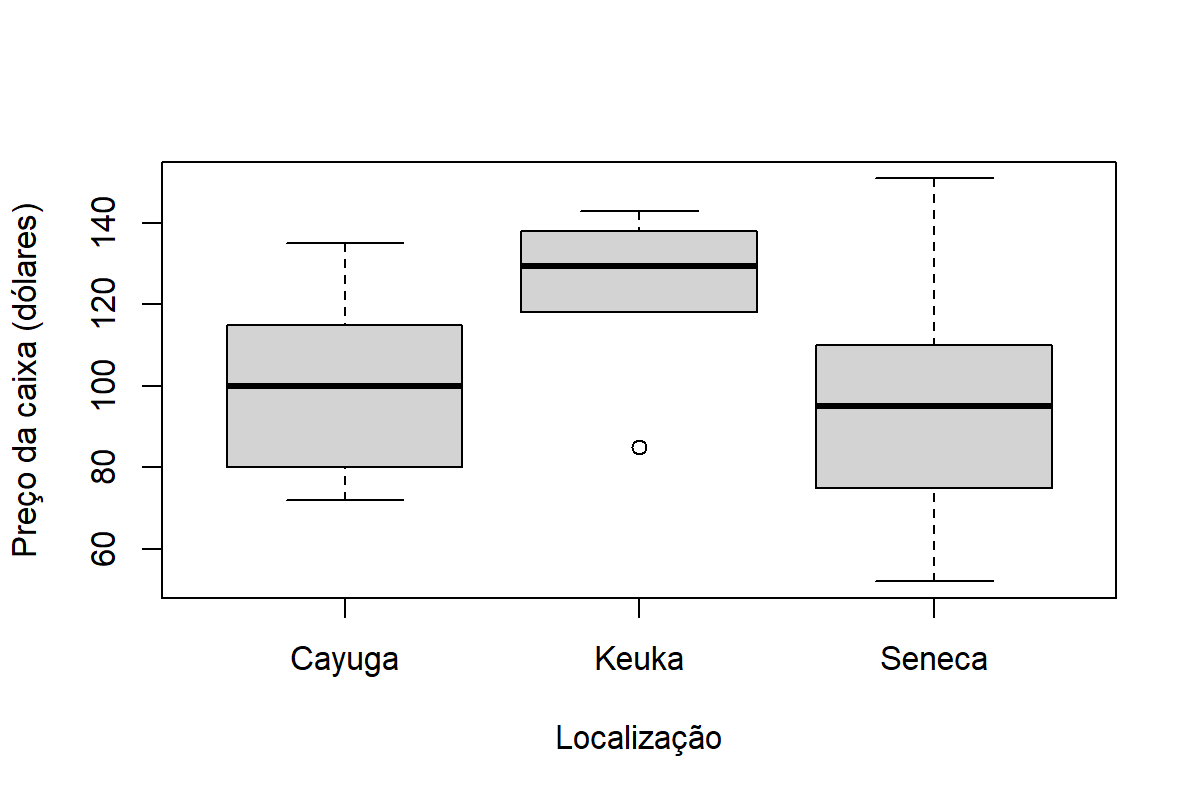
\includegraphics[width=.8\textwidth]{graficos_vinhedos} % Substitua pelo caminho da sua imagem
	\caption{Gráfico dos preços de caixas de vinho produzidos em três vinhedos no estado de Nova Iorque nos EUA.}
	\label{fig:graficos_vinhedos}
\end{figure}
	\begin{enumerate}
		\item Qual tipo de gráfico está sendo apresentado na Figura \ref{fig:graficos_vinhedos}? Quais são as variáveis utilizadas para preparar tal gráfico?
		\item Qual localização produz o vinho mais caro?
		\item Qual localização produz o vinho mais barato?
		\item Em qual localização os vinhos geralmente são mais caros?
		\item Descreva brevemente e compare a distribuição dos preços de vinho nas três regiões.
	\end{enumerate}
	
    \item Faça um rascunho de um histograma dos dados na Tabela~\ref{t:QI}.
	\begin{table}[htp]
	\centering
	\caption{Distribuição dos escores de QI das pessoas de uma determinada amostra. }
	\label{t:QI}
	\begin{tabular}{c|c}
	\hline
	QI & Frequência absoluta \\
	\hline
130–144 & 3 \\
115–129 & 11 \\
100–114 & 37 \\
85–99 & 34\\
70–84 & 16\\
65–69 & 2\\
\hline
Total & 103 \\
	\hline
	\end{tabular}
	\end{table}


	\item Os preços semanais de uma marca de pizza congelada foram coletados em duas cidades dos EUA durante três anos. Estatísticas descritivas desses dados são apresentadas na Tabela \ref{tab:preco_pizza}.	
	\begin{table}[htp]
	\centering
	\caption{Estatísticas descritivas dos preços (em dólares) semanais de pizza de uma certa marca. DP, Q1 e Q3 são, respectivamente, o desvio padrão, primeiro quartil e terceiro quartil.}
	\begin{tabular}{c|ccccccc}
	\hline
	Cidade & média & mediana & DP & min & max & Q1 & Q3 \\
	\hline
	Dallas & 2,62 & 2,61 & 0,1559 & 2,21 & 3,05 & 2,51 & 2,72 \\
	Chicago & 2,61 & 2,65 & 0,2122 & 1,55 & 3,03 & 2,53 & 2,74 \\
	\hline
	\end{tabular}
	\label{tab:preco_pizza}
	\end{table}
	
	Responda as perguntas a seguir com base nos resultados na Tabela \ref{tab:preco_pizza}.	
	\begin{enumerate}
	\item Calcule o desvio interquartílico dos preços em cada cidade.
	\item Há diferença na variabilidade dos preços de pizza dessas cidades? Justifique a sua resposta.
	\item Em qual cidade o preço da pizza tende a ser mais barato? Justifique a sua resposta.
	\end{enumerate}
	
	\item Uma equipe de psicólogos que estudava narcolepsia (um distúrbio do sono caracterizado por cochilos repentinos durante o dia) decidiu acompanhar 20 voluntários narcolépticos ao longo de um dia e registrar quantas vezes cada um deles adormeceu. Os dados coletados foram organizados na Tabela~\ref{t:narcolepsia}.
	\begin{table}[htp]
	\centering
	\caption{Distribuição dos números de cochilos dos 20 voluntários no estudo sobre narcolepsia. }
	\label{t:narcolepsia}
	\begin{tabular}{c|c}
	\hline
	Número de cochilos & Frequência absoluta \\
	\hline
7 & 2 \\
6 & 1\\
5 & 3\\
4 & 5\\
3 & 3\\
2 & 4\\
1 & 2\\
\hline
Total & 20 \\
	\hline
	\end{tabular}
	\end{table}
	
	Com base nos dados da Tabela~\ref{t:narcolepsia}, ache a moda, média e mediana do número de cochilos registrados na amostra.
	
	\item A Tabela~\ref{t:nivel_educacao} apresenta a distribuição de frequência dos níveis educacionais dos 39 funcionários administrativos de uma pequena empresa.
	\begin{table}[htp]
	\centering
	\caption{Distribuição do nível educacional dos funcionários administrativos de uma determinada empresa. }
	\label{t:nivel_educacao}
	\begin{tabular}{c|c}
	\hline
	Nível educacional & Frequência \\
	\hline
Pós-graduação & 3 \\
Ensino superior completo & 5\\
Ensino superior incompleto & 11\\
Ensino médio completo & 14\\
Ensino médio incompleto & 6\\
\hline
Total & 39 \\
	\hline
	\end{tabular}
	\end{table}
	
	Responda as perguntas a seguir com base nos resultados na Tabela \ref{t:nivel_educacao}.
\begin{enumerate}
	\item Qual é o tipo da variável \textit{Nível educacional}?
	\item Forneça uma medida de tendência central adequada para essa variável.	
\end{enumerate}			

	
		
	
\end{enumerate}


\end{document}